\section{Experiment P2C: matched-budget UWB link selection}
\subsection{Question and fair communication control}
P2B established that lowering the uniform all-six-link rate barely changes absolute fleet RMSE after the first positive rate, although relative-shape and worst-node errors continue to improve. P2C asks whether distributing a fixed number of pairwise UWB exchanges more intelligently among links can further reduce the errors that pairwise ranging can observe. The principal comparison is between link-selection policies at identical exchange times and capacity; P2B remains an equal-count but differently timed reference.

The simulator, \SI{60}{s} trajectories, \SI{100}{Hz} IMU and \SI{10}{Hz} UWB opportunity grid, 20 P2A seeds, noise realizations, initial-pose knowledge, and EKF are frozen. The three budgets are \(B\in\{180,360,720\}\) individual undirected range exchanges, matching the exchange counts of the P2B \(0.5,1,2\)~Hz all-link cases. Write \(s\in\{1,\ldots,600\}\) for the common UWB opportunities; all P2C policies are allocated the same number of exchanges at each opportunity:
\begin{equation}
    c_s=\left\lfloor\frac{sB}{600}\right\rfloor-
    \left\lfloor\frac{(s-1)B}{600}\right\rfloor.
    \label{eq:p2c_capacity}
\end{equation}
Thus \(\sum_s c_s=B\). The 180- and 360-exchange schedules activate one pair on 180 or 360 separate ticks. With 720 exchanges, 480 ticks activate one pair and 120 ticks activate two pairs. The opportunities and per-tick counts are fixed before observing measurements or running a selector. Each link is unique within its tick, so one pair is not ranged twice at the same opportunity.

This design controls the timing confound within P2C. In contrast, P2B spends each budget on widely separated rounds activating all six links simultaneously. Comparing a P2C policy with P2B at equal total counts evaluates the combination of timing and pair choice, not pair choice alone.

\subsection{Cyclic, random, geometry, and information policies}
The cyclic control walks through the six undirected pairs in a fixed order across successive exchanges. The random control samples distinct pairs uniformly at each tick with a dedicated scheduling random stream. Its sensor observations and initialization remain matched to the other policies, while its link decisions are independent of the sensor-noise random numbers.

The geometry policy uses only the EKF-predicted node positions and past selections. Each predicted pair defines a range-direction Jacobian \(\bm h_{ij}\) over the eight planar position components. A geometry Gramian \(G\) sums the outer products of previous selected range rows, with an exponential \SI{2}{s} memory. At each choice it maximizes the regularized marginal geometry score
\begin{equation}
    q_{ij}^{\mathrm{geom}} =
    \frac{\bm h_{ij}^{\top}}{\sigma_r}
    \bigl(G+I\bigr)^{-1}
    \frac{\bm h_{ij}}{\sigma_r},
    \qquad \sigma_r=\SI{0.12}{m}.
\end{equation}
The unit regularizer and memory are fixed before evaluation. When two links are permitted, the first selected row is added to a temporary Gramian before scoring the second. This is a geometric-diversity heuristic: it considers relative range directions without using estimator uncertainty.

The information policy uses the EKF's predicted joint covariance \(P^-\). For a candidate with full-state Jacobian \(H_{ij}\), define
\begin{equation}
    \bm v_{ij}=P^-H_{ij}^{\top},\quad
    S_{ij}=H_{ij}P^-H_{ij}^{\top}+\sigma_r^2,\quad
    q_{ij}^{\mathrm{info}}=
    \frac{\|C\bm v_{ij,p}\|_2^2}{4S_{ij}},
\end{equation}
where \(\bm v_{ij,p}\) contains its eight position entries and \(C=I_8-(\bm1_4\bm1_4^\top/4)\otimes I_2\) removes common translation. The score is the predicted reduction in the mean centered relative-position covariance trace. If two links are permitted, a hypothetical covariance update for the first selected link precedes scoring of the second. Both adaptive policies make their decision \emph{after inertial prediction and before reading the current range}. They do not use truth or the noisy range to choose a pair.

For each seed and budget we report whole-run fleet, worst-node, centroid, and relative-shape position RMSE, accompanied by per-link use counts and time-resolved error histories. In addition to mean and sample standard deviation across 20 seeds, paired differences against cyclic and random quantify whether a selector is consistently better for the same sensor realization and schedule. Range count is a proxy for communication effort; radio energy and packet overhead are not measured.

\subsection{Matched-seed results and interpretation}
Table~\ref{tab:p2c_results} summarizes the complete 20-seed campaign. The three rate-equivalent budgets correspond to 5\%, 10\%, and 20\% of the P2A full UWB exchange count. Within each budget the policies have exactly the same exchange count at \emph{every} tick, so the four policy rows constitute a matched link-choice comparison. In particular, a precomputed potential range measurement has the same noisy value whenever two policies select the same pair at the same time in a matched seed.

\begin{table}[htbp]
    \centering
    \caption{P2C 20-seed localization results. Fleet and relative-shape RMSE are across-seed means \(\pm\) sample standard deviations of whole-run RMSE; worst-node values are across-seed means. All errors are in metres.}
    \label{tab:p2c_results}
    \begin{tabular}{rlrrr}
        \toprule
        Exchanges & Link policy & Fleet RMSE & Worst-node RMSE & Shape RMSE \\
        \midrule
        180 & Cyclic & \(1.0639\pm0.4476\) & 1.0990 & \(0.1095\pm0.0158\) \\
            & Random & \(1.0639\pm0.4468\) & 1.1058 & \(0.1174\pm0.0251\) \\
            & Geometry & \(1.0635\pm0.4462\) & 1.0910 & \(0.1066\pm0.0204\) \\
            & Information & \(1.0637\pm0.4480\) & 1.0889 & \(0.1068\pm0.0201\) \\
        \midrule
        360 & Cyclic & \(1.0610\pm0.4484\) & 1.0855 & \(0.0824\pm0.0159\) \\
            & Random & \(1.0621\pm0.4486\) & 1.0960 & \(0.0914\pm0.0188\) \\
            & Geometry & \(1.0607\pm0.4490\) & 1.0856 & \(0.0853\pm0.0165\) \\
            & Information & \(1.0603\pm0.4499\) & 1.0831 & \(0.0789\pm0.0141\) \\
        \midrule
        720 & Cyclic & \(1.0594\pm0.4496\) & 1.0755 & \(0.0687\pm0.0143\) \\
            & Random & \(1.0593\pm0.4507\) & 1.0752 & \(0.0697\pm0.0105\) \\
            & Geometry & \(1.0598\pm0.4503\) & 1.0801 & \(0.0673\pm0.0107\) \\
            & Information & \(1.0593\pm0.4504\) & 1.0738 & \(0.0682\pm0.0109\) \\
        \bottomrule
    \end{tabular}
\end{table}

Figure~\ref{fig:p2c_budget} displays all three budgets beside the equal-count P2B all-link reference. The measured fleet-centroid RMSE remains between about \SI{1.055}{m} and \SI{1.057}{m} for every P2C condition, and fleet RMSE varies little between link policies at the same budget. The differentiated outcomes are the relative-shape and worst-node errors. At 360 exchanges the information policy reaches \SI{0.0789}{m} mean shape RMSE, compared with \SI{0.0824}{m} for cyclic and \SI{0.0914}{m} for random. These differences correspond to approximately 4.3\% and 13.7\% lower mean shape RMSE, respectively. At 180 exchanges the geometry and information policies have similar shape RMSE (\SI{0.1066}{m} and \SI{0.1068}{m}); cyclic is \SI{0.1095}{m}. At 720 exchanges the shape results converge near \SI{0.067}{m}--\SI{0.070}{m}, and no one policy is consistently best across all metrics.

\begin{figure}[htbp]
    \centering
    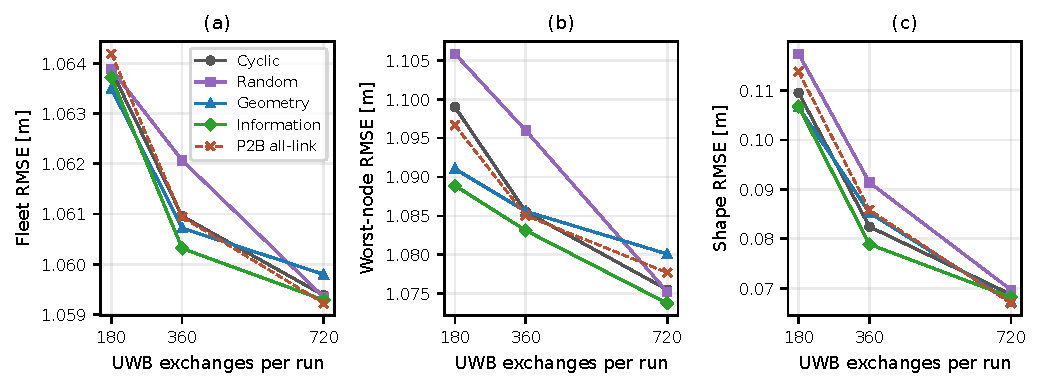
\includegraphics[width=0.98\textwidth]{figures/phase2/p2c_budget_tradeoff.pdf}
    \caption{P2C 20-seed means versus individual pairwise UWB exchanges for (a) absolute fleet, (b) worst-node, and (c) centered relative-shape RMSE. P2B all-link results at matching total exchange counts are shown for context; their exchange timing differs from P2C and therefore cannot isolate a link-selection effect. Across-seed variability and within-seed policy differences are presented separately in Table~\ref{tab:p2c_results} and Fig.~\ref{fig:p2c_paired}.}
    \label{fig:p2c_budget}
\end{figure}

Figure~\ref{fig:p2c_paired} subtracts each seed's cyclic result before aggregation, removing much of the between-seed difficulty variation. Error bars represent one sample standard deviation of the \emph{paired differences}, not standard deviations of the raw RMSEs or confidence intervals. At 360 exchanges the information-minus-cyclic mean shape difference is \(-0.00356\pm0.01174\)~m, favoring information in 13 of 20 matched seeds. Against random, the corresponding difference is \(-0.01250\pm0.01677\)~m and information wins in 17 of 20 seeds. A descriptive paired-seed bootstrap (30,000 resamples, percentile 95\% intervals) gives \([-0.00859,0.00144]\)~m against cyclic and \([-0.01953,-0.00517]\)~m against random. Thus the evidence for improving on random is clearer at this budget; the 20 seeds do not establish a consistent information-over-cyclic shape advantage. These intervals describe stochastic realizations of the \emph{fixed} trajectories and were not adjusted for comparing multiple policies and budgets.

\begin{figure}[htbp]
    \centering
    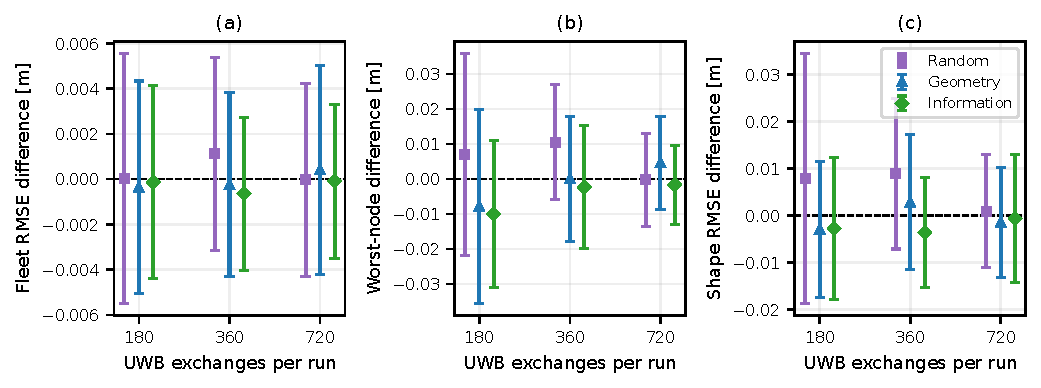
\includegraphics[width=0.98\textwidth]{figures/phase2/p2c_paired_differences.pdf}
    \caption{Paired P2C policy-minus-cyclic whole-run RMSE differences across 20 matched seeds. Markers show the mean and error bars show one sample standard deviation of the 20 paired differences. Values below zero favor the named policy; zero is equal performance. Large raw fleet-RMSE variability is largely common to paired runs.}
    \label{fig:p2c_paired}
\end{figure}

The adaptive policies do choose a different mix of links. Figure~\ref{fig:p2c_usage} compares mean link-use fractions. Cyclic is exactly balanced at one sixth per pair. At 360 exchanges, information selects pairs 1--3 and 3--4 for about 19.8\% and 20.4\% of its exchanges and pair 2--3 for about 12.7\%. Geometry makes a milder redistribution. No candidate link is permanently excluded; these observed fractions are specific to the chosen paths, estimator uncertainty, and geometry-memory setting.

\begin{figure}[htbp]
    \centering
    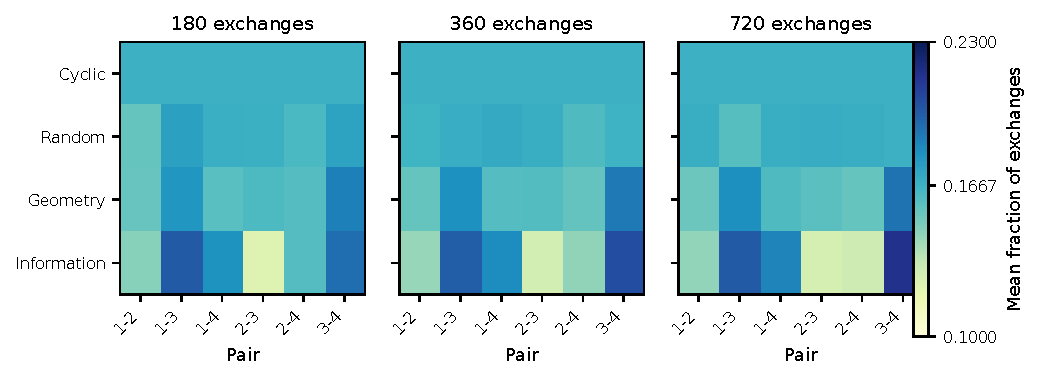
\includegraphics[width=0.98\textwidth]{figures/phase2/p2c_link_usage.pdf}
    \caption{Mean fraction of a run's exchanges assigned to each undirected pair, averaged over the 20 seeds. The color scale zooms to 10\%--23\% to resolve differences around the balanced 16.7\% allocation; color differences do not imply a change in total exchange count.}
    \label{fig:p2c_usage}
\end{figure}

Figure~\ref{fig:p2c_time} resolves the shape error through time at the lowest and highest P2C budgets. Each trace is the across-seed pointwise mean of the instantaneous centered relative-shape RMS error. The translucent band is one pointwise sample standard deviation clipped at zero, not a confidence interval for the mean. The policies share the early error rise and differ modestly thereafter; at 720 exchanges the traces largely overlap. The whole-run paired comparisons, rather than a visually selected time interval, support the policy conclusion.

\begin{figure}[htbp]
    \centering
    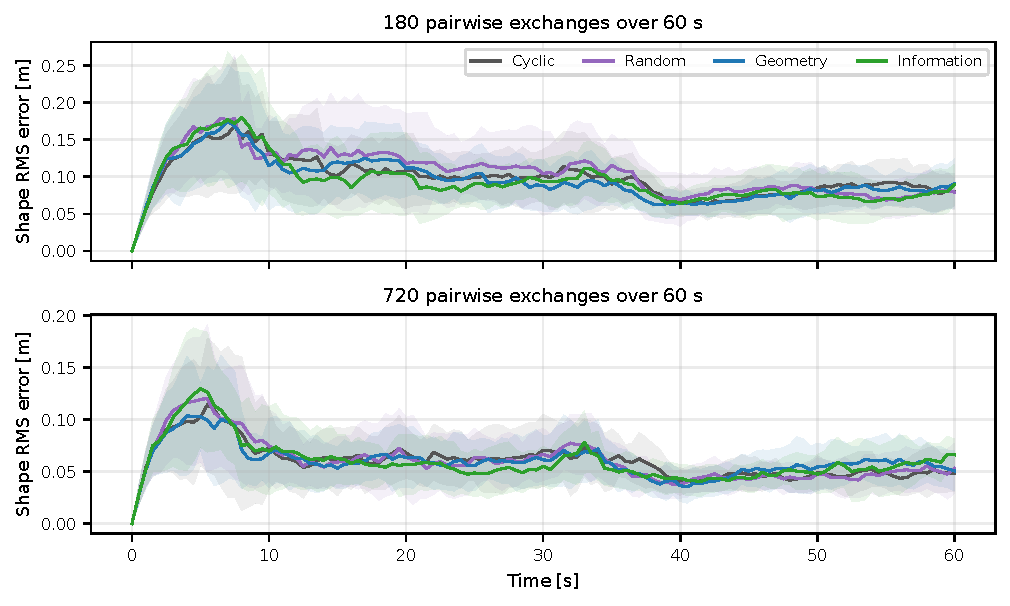
\includegraphics[width=0.98\textwidth]{figures/phase2/p2c_time_profiles.pdf}
    \caption{P2C relative-shape error histories at 180 and 720 exchanges. Curves show pointwise means over 20 matched seeds and shading shows mean \(\pm\) one sample standard deviation, clipped at zero. The fixed time allocation is identical for all four policies within each panel.}
    \label{fig:p2c_time}
\end{figure}

\subsection{P2C decision and handoff}
P2C demonstrates a measurable but budget-dependent scope for pair selection. Information-based selection is most promising at the intermediate 360-exchange budget relative to random scheduling, whereas a simple cyclic rotation is already competitive and the geometric-diversity heuristic does not consistently improve upon it. None of the selectors reduces the unobservable common translation, so absolute fleet RMSE remains close to the P2B error floor despite clearer differences in relative shape and worst-node error. A more complex policy should therefore be justified against \emph{cyclic}, not solely against random.

The comparison has three important bounds: the geometric-memory setting was fixed without a parameter study, covariance-based scores rely on the current EKF model, and one fixed trajectory set was repeated under 20 noise seeds. P2D next examines missed and corrupted ranging on matched schedules, counts attempted and successful exchanges separately, and tests whether any P2C preference persists when range availability and quality vary. These ideal-Gaussian P2C results do not yet justify selecting a permanent link policy for physical radios.
